\documentclass[UTF8, letter]{article}

\usepackage[margin=1in]{geometry}
\usepackage{graphicx}
\usepackage{lipsum}
\usepackage[framemethod=tikz]{mdframed}
\usepackage{minted}
\usepackage{setspace}
\usepackage{xcolor}
\usemintedstyle{xcode}

\definecolor{codebg}{RGB}{192,199,209}

\mdfdefinestyle{codeframe}{
	backgroundcolor=codebg,
	linewidth=0,
	skipbelow=-10,
}
\newmdenv[style=codeframe,%
	settings={\singlespacing}]{codeblock}

\title{Programming Assignment 1 \\
\large INFO-5502 (Section 002): \\
Analytic Tools, Techniques and Methods }
\author{Ramandeep Harjai}



\begin{document}
\maketitle

\doublespacing
\setlength{\parskip}{\baselineskip}
\setlength{\parindent}{4em}

Write a Python program that can take strings of different lengths - each string may include digits, characters, and special symbols - and then sort them - you can use any sorting algorithm that interests you.  You need to define the rule for sorting and then implement the sorting function using Python - DO NOT use any existing sort function from either Python or an external module - that is, program the "sort" algorithm yourself.  Using Python, visualize a list of input strings - the list must include at least 500 strings of differing lengths.   Use a scatter plot to do the visualization - one dimension will be the length of each string - and the other dimension could be the order of the string in the list.

Your submission should include the following:

1) Submit the python program with a brief description of how the program works (3 points);  2)  A description that specifically describes how the sorting rule works (3 points);  3)  Visualization results and testing results with 5 test cases -  the 5 test cases would consist of 5 lists of 500 strings of differing lengths (4 points).

These strings can come from any source that is of interest to you -  e.g. favorite book,   Wikipedia,  Twitter data - you can use strings from any source that interests you - you just need string data from somewhere.

\pagebreak
\paragraph{List of Random Phrases}
The python function: \texttt{randomStringGenerator}, generates a list of random phrases. Each phrase is generated using 1 to 5 words (randomly), where each word is made up of 1 to 12 alpha-numeric characters (randomly). The function accepts an argument: \texttt{numStrings} --- total number of strings (or phrases) to be generated, and returns a \texttt{List[]} of size: \texttt{numStrings}.

\begin{codeblock}
\begin{minted}{python}
def randomStringGenerator(numStrings:int)->[]:
  """ generates & return a list of random strings
  """
  lstStr = []         # list to hold random strings
  minPhraseLen = 1    # minimum number of words in Random Phrase
  maxPhraseLen = 5    # maximum number of words in Random Phrase
  minStrLen = 1       # minimum length for the random string
  maxStrLen = 12      # maximum length for the random string
  for _ in range(numStrings):
    rndPhraseLen = randint(minPhraseLen, maxPhraseLen)
    rndPhrase = ""
    for i in range(rndPhraseLen):
      rndLen = randint(minStrLen, maxStrLen)
      if _%5 == 0:
        # use alphabets and numbers
        rndPhrase += ''.join(choices(string.ascii_uppercase + string.digits,
                                     k = randint(minStrLen, maxStrLen)))
      elif _%9 == 0:
        # use alphabets, numbers, and special characters
        rndPhrase += ''.join(choices(string.ascii_uppercase + string.digits + 
                                     string.punctuation, 
                                     k = randint(minStrLen, maxStrLen)))
      else:
        # use alphabets only
        rndPhrase += ''.join(choices(string.ascii_uppercase,
                                     k = randint(minStrLen, maxStrLen)))
        
      rndPhrase += " "
    lstStr.append(rndPhrase)
  return lstStr	
\end{minted}
\end{codeblock}

\vspace{5mm}
\begin{codeblock}[frametitle=Output --- List of Random Phrases:]
\begin{minted}{python}
['4FXMRH ', 'NHAYCZ V UVJOUWEU I INOOK ', 'C NRNAEGAUV VFFG HDJ DQMIDPY ', 
'DGLYZ EKH RMOGMF JVUFP ', 'WMXLXNZSKJGP GD ', 'LJMEXHDFHTFJ 7ABCB FZ7Q39FT2 12X3JR ', 
'KHMKA AL DG U ZFVO ', 'CALCFHCZX VRWZLTOPXX ', 'MDMYBR SSDER ', '=\$=? ', 'Z2 FB ', 
'E ', 'ULGAIJXON JWRCDC ZBDHPTMZD ', 'GEVSGK TFRPRVUYUYM ', 'HBWHTSU UVAMVENCYWSQ ', 
'5G A81 ', 'KLUQOZUANFI SPB AAFWZO GAUIBZIE EMXYSJVNA ', ...]	
\end{minted}
\end{codeblock}

\pagebreak
\paragraph{ASCII Score}
The python function: \texttt{stringAsciiScore}, returns the ASCII score of a string, which is a total of ASCII values of all characters in the string. The function accepts a parameter: \texttt{strg} --- string for which the ASCII score needs to be computed, and returns \texttt{int} --- numeric value of ASCII score.

\begin{codeblock}
\begin{minted}{python}
def stringAsciiScore(strg:str)->int:
  """ compute and return the ascii score for a given string
      ascii score of a string = total of ascii scores 
                                of all characters in the string
  """
  asciiScore = 0
  if not strg:
    return asciiScore
  for _ in range(len(strg)):
    asciiScore += ord(strg[_])
  return asciiScore
\end{minted}
\end{codeblock}

\vspace{5mm}
\begin{codeblock}[frametitle=Output --- ASCII Score:]
\begin{minted}{python}
>> 'A' (input)
65 (output)
\end{minted}
\end{codeblock}

\vspace{5mm}
\begin{codeblock}[frametitle=Output --- ASCII Score:]
\begin{minted}{python}
>> '$' (input)
36 (output)
\end{minted}
\end{codeblock}

\vspace{5mm}
\begin{codeblock}[frametitle=Output --- ASCII Score:]
\begin{minted}{python}
>> 'Hello World!' (input)
1085 (output)
\end{minted}
\end{codeblock}

\vspace{5mm}
\begin{figure}[h!]
  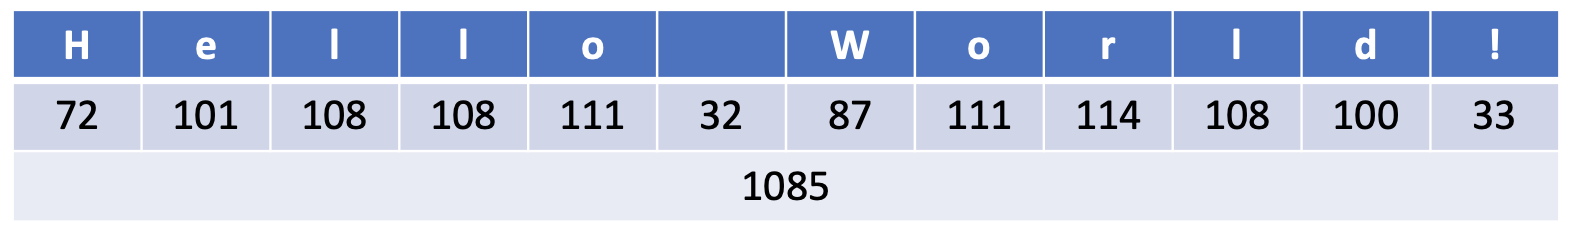
\includegraphics[width=\linewidth]{ascii_score.png}
  \caption{Compute ASCII Score for 'Hello World!'}
  \label{fig:boat1}
\end{figure}


\pagebreak
\paragraph{Sorting}
The python function: \texttt{bubbleSort}, returns a sorted string where all characters in the string are sorted in ascending order of their ASCII values. The function uses \texttt{bubble sort algorithm} to the sort the list. The function accepts a parameter: \texttt{strg} --- string to be sorted, and returns \texttt{str} --- sorted string.

\begin{codeblock}
\begin{minted}{python}
def bubbleSort(strg:str)->str:
  """ sort list using bubble sort algorithm """
  if (not strg):
    return ""

  strgSortedList = list(strg)
  strgLen = len(strgSortedList)  
  for i in range(strgLen):
    for j in range (strgLen-i-1):
      # compare the ascii values of two characters
      # character with smaller ascii value will precede the other character  
      if stringAsciiScore(strgSortedList[j]) > stringAsciiScore(strgSortedList[j+1]):
        strgSortedList[j], strgSortedList[j+1] = strgSortedList[j+1], strgSortedList[j]
        
  return "".join(strgSortedList) 
\end{minted}
\end{codeblock}

\vspace{5mm}
\begin{codeblock}[frametitle=Output --- Sorting:]
\begin{minted}{python}
>> 'LJMEXHDFHTFJ 7ABCB FZ7Q39FT2 12X3JR' (input: phrase)
'   12233779ABBCDEFFFFHHJJJLMQRTTXXZ' (output: sorted string)
\end{minted}
\end{codeblock}

\vspace{5mm}
\begin{figure}[h!]
	\centering
	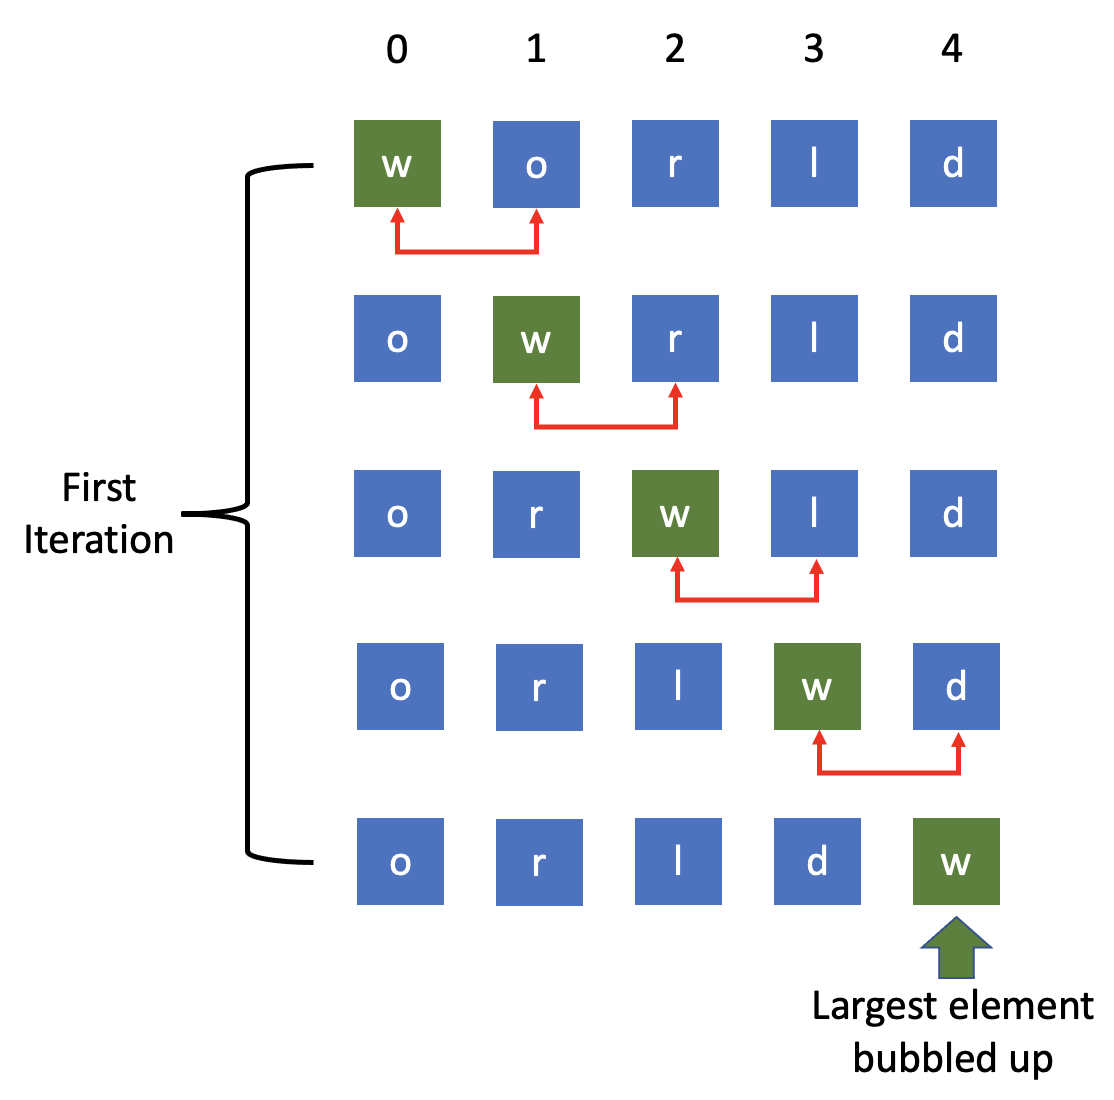
\includegraphics[width=0.5\linewidth]{bubble_sort.png}
	\caption{Bubble Sort Algorithm --- First Iteration}
	\label{fig:boat1}
\end{figure}


\pagebreak
\paragraph{Sorting (List)}
The python function: \texttt{bubbleSortList}, returns a sorted list where all elements in the list are sorted in ascending order of their Length and ASCII values. The function uses \texttt{bubble sort algorithm} to the sort the list. The function accepts a parameter: \texttt{lst} --- list of strings (or phrases), and returns \texttt{List[]} --- sorted list.

\begin{codeblock}
\begin{minted}{python}
def bubbleSortList(lst:list)->list:
  """ sort list using bubble sort algorithm """
  if (not lst) or (len(lst)<=0):
    return []

  sortedList = lst.copy()
  lstLen = len(sortedList)
  for i in range(lstLen):
    for j in range (lstLen-i-1):
      # compare by string length
      # shorter length string should preceed longer length string
      if len(sortedList[j]) > len(sortedList[j+1]):
        sortedList[j], sortedList[j+1] = sortedList[j+1], sortedList[j]
      
      # for same length strings
      # compare the total ascii values of two string
      # string with smaller total ascii value will preceed the other string
      if len(sortedList[j]) == len(sortedList[j+1]):  
        if stringAsciiScore(sortedList[j]) > stringAsciiScore(sortedList[j+1]):
          sortedList[j], sortedList[j+1] = sortedList[j+1], sortedList[j]

  return sortedList
\end{minted}
\end{codeblock}

\vspace{5mm}
\begin{codeblock}[frametitle=Output --- Sorting (List):]
\begin{minted}{python}
>> ['P 1K3SV', 'VEAPH HMBOGGWBW ZXZJC OJTWXCEDYRGM BVE', 
'ZPQKFEDD DIAUAZFNW J CAAEPI LVAIISGVHBR', 'FDUEZUNB', 'KFEA', 
'QVCDIA5OL', 'S LBGX', 'GY XCYFG VKWPGIICBYD', 'NT VPQT XCPLQH DA', 
'*W4P +$C>4P[9'] (input: list)

['KFEA', 'S LBGX', 'P 1K3SV', 'FDUEZUNB', 'QVCDIA5OL', 
'*W4P +$C>4P[9', 'NT VPQT XCPLQH DA', 'GY XCYFG VKWPGIICBYD', 
'VEAPH HMBOGGWBW ZXZJC OJTWXCEDYRGM BVE', 
'ZPQKFEDD DIAUAZFNW J CAAEPI LVAIISGVHBR'] (output: sorted list)
\end{minted}
\end{codeblock}



\pagebreak
\paragraph{Program Execution}
The python program starts with creating a list of 500 random phrases, using \texttt{randomStringGenerator()}. Program then iterates through each element of the list. Each element is sorted with the \texttt{bubble sort algorithm}, using the \texttt{bubbleSort()} function. Next, the program sorts the list itself, with the \texttt{bubble sort algorithm}, using the \texttt{bubbleSortList()} function. Finally, the program creates two scatter charts --- (1) for list with sorted elements, and (2) for sorted list of sorted elements. Scatter charts are created using \texttt{matplotlib} module.

\begin{codeblock}
\begin{minted}{python}
# generate list of random strings
maxStrings = 500
lstRndStrg = randomStringGenerator(maxStrings)

print(len(lstRndStrg), "Random Strings: ", lstRndStrg)
\end{minted}
\end{codeblock}

\vspace{5mm}
\begin{codeblock}
\begin{minted}{python}
# sort each element of the list
lstRndStrgSorted = []
for _ in range(len(lstRndStrg)):
  lstRndStrgSorted.append(bubbleSort(lstRndStrg[_]))

print(len(lstRndStrgSorted), "Random Strings (Sorted Elements): ", lstRndStrgSorted)
\end{minted}
\end{codeblock}

\vspace{5mm}
\begin{codeblock}
\begin{minted}{python}
# sort entire list
lstRndStrgSorted2 = bubbleSortList(lstRndStrgSorted)
print(len(lstRndStrgSorted2), "Random Strings (Sorted List & Elements): ", 
	lstRndStrgSorted2)
\end{minted}
\end{codeblock}

\vspace{5mm}
\begin{codeblock}
\begin{minted}{python}
# Plot
fig, (ax1, ax2) = plt.subplots(1,2,constrained_layout=True)
fig.set_size_inches(12, 6)
fig.set_dpi(100)
fig.suptitle('Scatter Plots of Unsorted & Sorted List of Random Strings')

# Scatter (sub)Plot for Unsorted List
ax1.set_title('List with Sorted Elements')
ax1.set(xlabel='Position of Random String in the List', 
        ylabel='Length of Random String')
ax1.scatter([range(len(lstRndStrgSorted))], 
            [len(strg) for strg in lstRndStrgSorted])

# Scatter (sub)Plot for Sorted List
ax2.set_title('Sorted List with Sorted Elements')
ax2.set(xlabel='Position of Random String in the List', 
        ylabel='Length of Random String')
ax2.scatter([range(len(lstRndStrgSorted2))], 
            [len(strg) for strg in lstRndStrgSorted2])
\end{minted}
\end{codeblock}

\pagebreak
\section*{Output: 5 test cases}

\begin{figure}[hbt!]
	\centering
	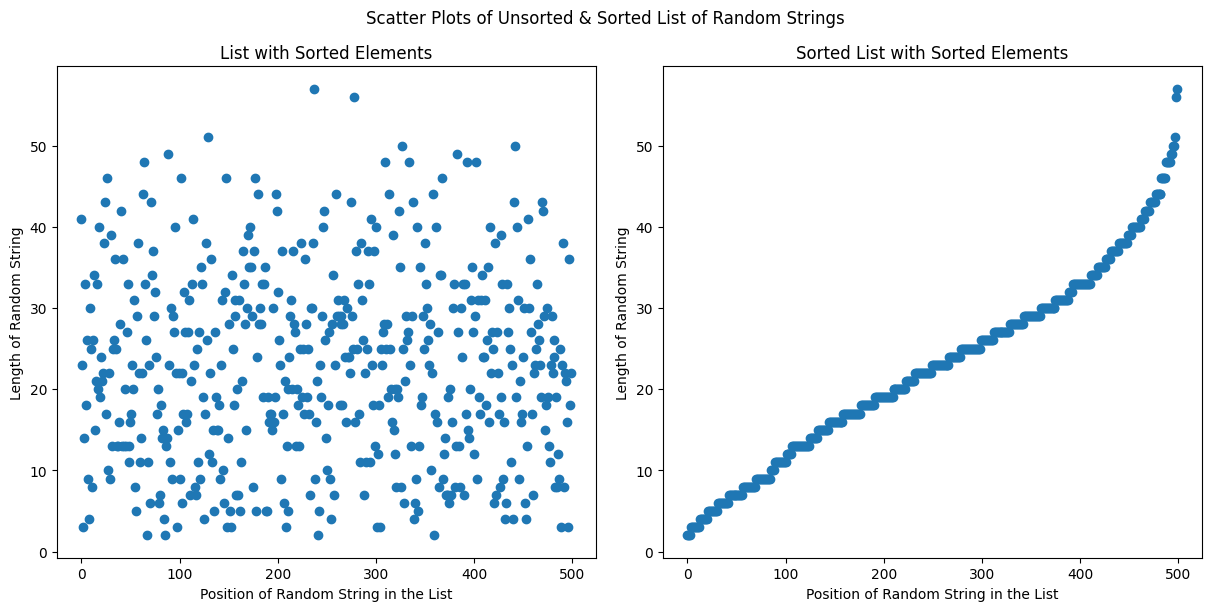
\includegraphics[width=\linewidth]{output_1.png}
	\caption{Output 1}
	\label{fig:Output1}
\end{figure}

\vspace{5mm}
\begin{figure}[hbt!]
	\centering
	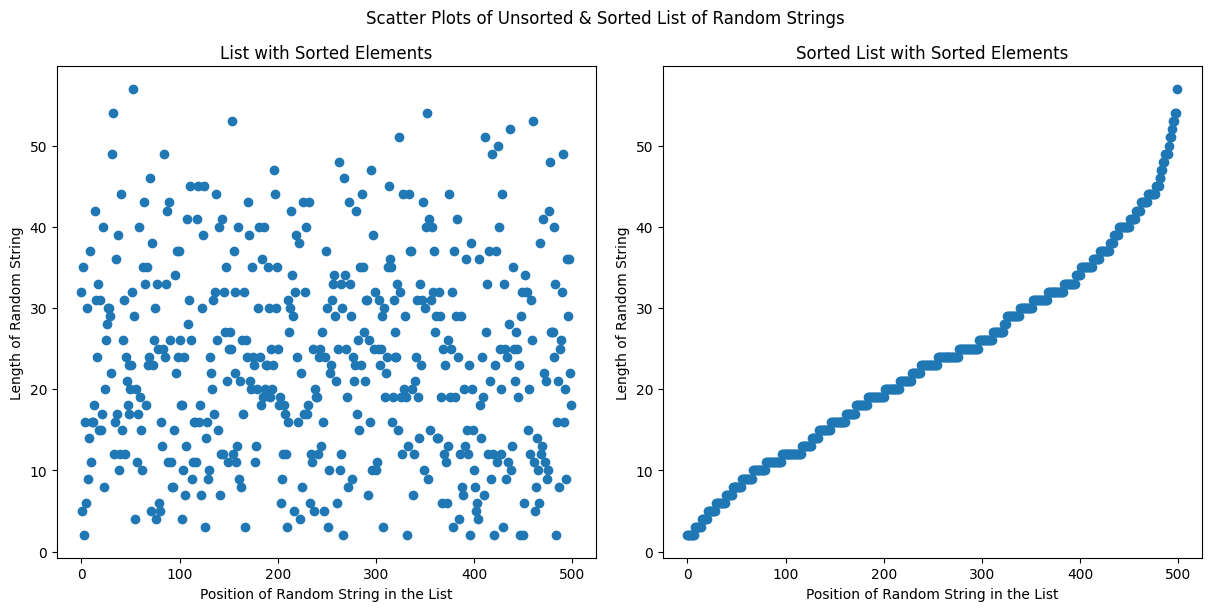
\includegraphics[width=\linewidth]{output_2.png}
	\caption{Output 2}
	\label{fig:Output2}
\end{figure}

\vspace{5mm}
\begin{figure}[hbt!]
	\centering
	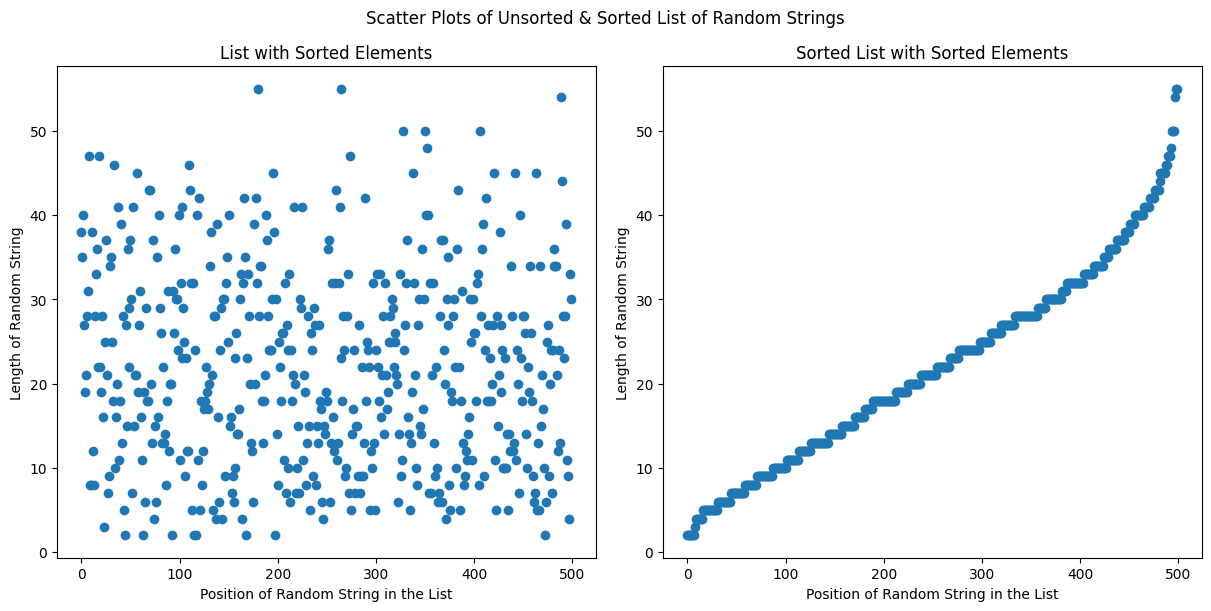
\includegraphics[width=\linewidth]{output_3.png}
	\caption{Output 3}
	\label{fig:Output3}
\end{figure}

\vspace{5mm}
\begin{figure}[hbt!]
	\centering
	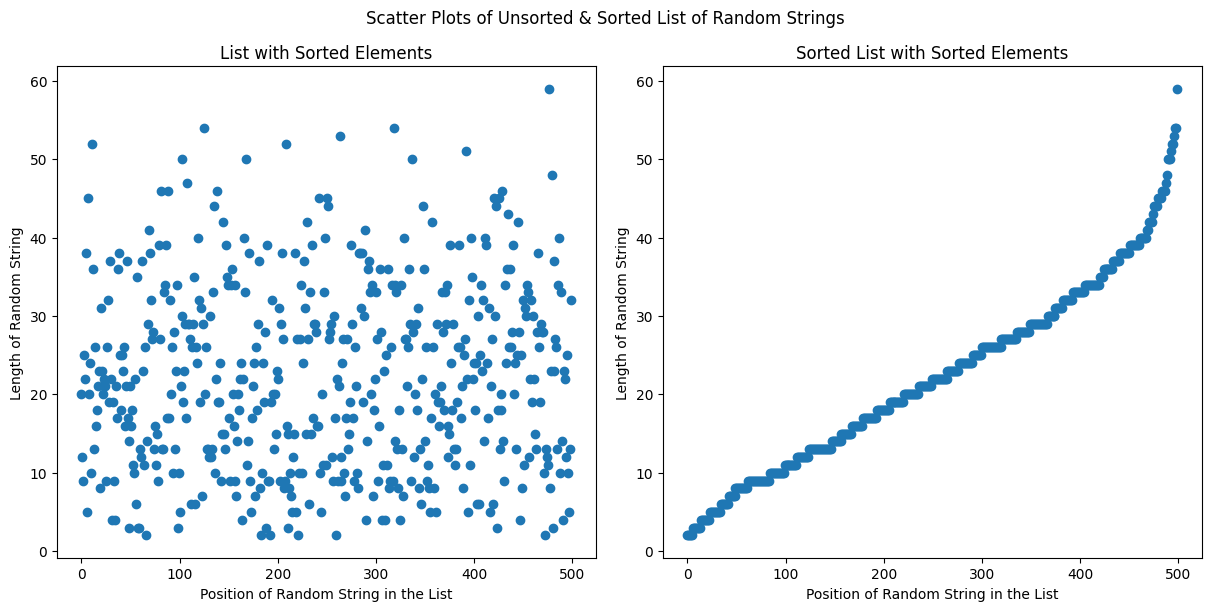
\includegraphics[width=\linewidth]{output_4.png}
	\caption{Output 4}
	\label{fig:Output4}
\end{figure}

\vspace{5mm}
\begin{figure}[hbt!]
	\centering
	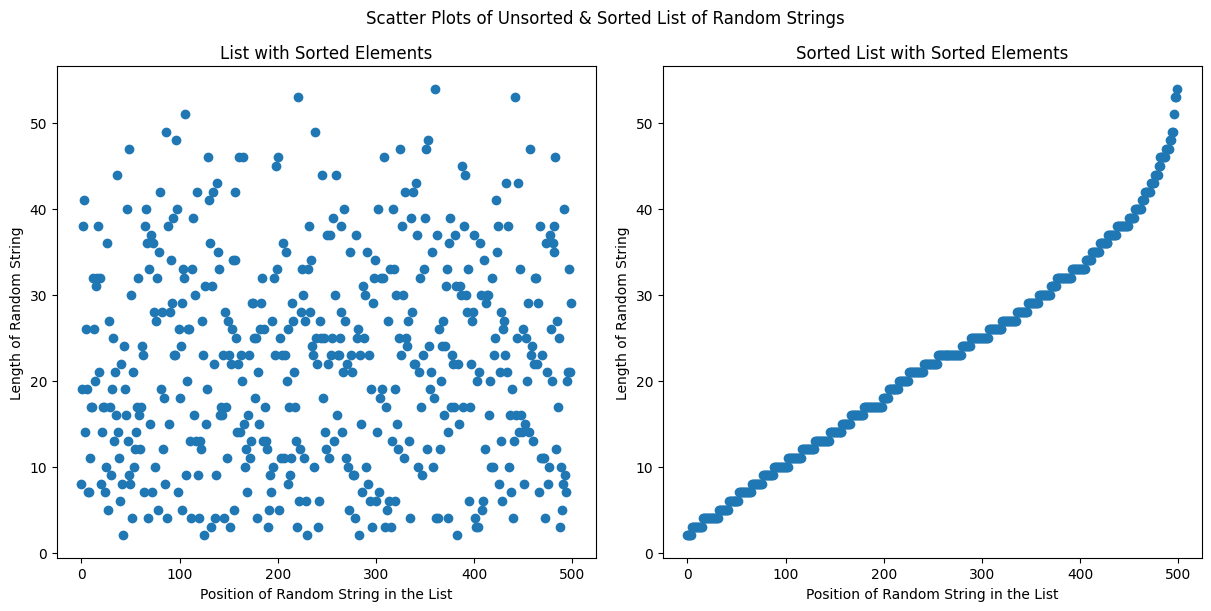
\includegraphics[width=\linewidth]{output_5.png}
	\caption{Output 5}
	\label{fig:Output5}
\end{figure}


	
\end{document}
